\chapter{From Spike Trains to Node Embeddings: Solving the Reservoir-to-Graph Representation Problem}
\label{chap:embeddings}

\section{Introduction: The Representation Bottleneck at the Heart of ARSPI-Net}
\label{sec:ch4_intro}

With the operating regime established, the question becomes what temporal structure survives the reservoir-to-embedding compression and what is discarded---the bottleneck problem that determines how much of the revealed order is preserved in usable form. This is simultaneously a compression question and an interpretability question: the coding scheme must not only preserve discriminative information but must do so in a form where each feature maps onto a named temporal property of the reservoir's response. A representation that achieves high accuracy but whose features are uninterpretable---as occurs with raw spike-train statistics or learned latent spaces---would violate the intrinsic interpretability requirement established in Chapter~\ref{chap:introduction} (Section~\ref{sec:inverse_problem}).

The research gap identified in Chapter~\ref{chap:background} (Section~\ref{sec:research_gap}) is precise: there is no established, rigorously validated methodology for transforming the output of a spiking reservoir into a representation suitable for graph neural network inference. This is not a minor implementation detail. It is the central methodological problem of the dissertation, because the entire ARSPI-Net architecture depends on the quality of the bridge between its two computational stages. If the node embeddings produced by the LSM front end do not preserve the temporal structure that the reservoir extracts, or if they introduce artifacts that confound the graph model's relational learning, then no amount of sophistication in the GNN back end can compensate. The representation bottleneck between reservoir and graph is the critical design point of the architecture.

Chapter~\ref{chap:lsm} established that the reservoir, at the validated operating point ($\beta = 0.05$, $M_{\text{th}} = 0.5$), produces stable, graded, spike-based responses whose discriminative content is concentrated in the early post-stimulus window. However, that chapter used the coarsest possible feature representation---the mean firing rate---and evaluated it on a deliberately simple amplitude discrimination task. What remains to be determined is how to engineer a representation that preserves the reservoir's temporal structure with sufficient fidelity for the downstream graph model while satisfying the practical constraints of dimensionality, robustness, and interpretability.

The raw output of the reservoir for a single trial and a single EEG channel is a binary spike train matrix $\mathbf{S} \in \{0, 1\}^{N_{\text{res}} \times T}$, where $N_{\text{res}} = 256$ neurons and $T = 60$ time steps in the adopted feature window (steps 10--70). This is a 15,360-element binary spatiotemporal object---sparse, high-dimensional, and structured in both space (across neurons) and time (across steps). A GNN requires a dense, fixed-length feature vector $\mathbf{h}_v^{(0)} \in \mathbb{R}^d$ for each node $v$. The transformation from $\mathbf{S}$ to $\mathbf{h}_v^{(0)}$ determines what aspects of the reservoir's driven response are preserved for the graph model and what aspects are discarded.


\section{Theoretical Background: The Neural Coding Problem}
\label{sec:neural_coding_theory}

The question of how to extract a feature vector from a spike train is a specific instance of the \emph{neural coding problem}---one of the foundational questions in computational neuroscience. The debate concerns what aspects of a neural spike train carry information about the stimulus: the overall firing rate (rate coding), the precise timing of individual spikes (temporal coding), or some combination \cite{gerstner_spiking_2002, dayan2001, Rieke1997}.

This debate is directly relevant to the ARSPI-Net embedding problem. If the reservoir's discriminative information is entirely captured by the firing rate, then the mean firing rate (MFR) is a sufficient representation and no finer temporal resolution is needed. If, however, the information is distributed across the temporal profile of the spiking response, the MFR will discard task-relevant structure.

From a statistical perspective, the ideal feature extraction would produce a \emph{sufficient statistic} for the classification task: a function $T(\mathbf{S})$ that preserves all information about the class label $y$. The data processing inequality guarantees that $I(y; T(\mathbf{S})) \leq I(y; \mathbf{S})$, with equality if and only if $T$ is sufficient. The coding scheme comparison in this chapter is therefore an empirical assessment of how close different summary statistics come to sufficiency. This connects to the information bottleneck principle \cite{tishby_deep_2015}, which formalizes the trade-off between compression and relevance that the BSC$_6 \to$ PCA-64 pipeline must navigate.

\subsection{A Diagnostic Task: Temporal Pattern Discrimination}

To probe the rate-versus-temporal coding question, this chapter uses a controlled task specifically designed so that the two stimulus classes are indistinguishable by their total energy but distinguishable by their temporal structure. Class~0 (``early burst'') presents three sub-pulses with a strong--medium--weak amplitude profile; Class~1 (``late burst'') reverses this to weak--medium--strong. Both classes have approximately equal total energy within the analysis window, ensuring that any classifier operating on total spike counts (i.e., a rate code) cannot distinguish them. Additive Gaussian noise ($\sigma = 0.5$), amplitude jitter ($\pm 30\%$), and timing jitter ($\pm 5$ steps) are applied to create inter-trial variability. This task is more demanding than the Chapter~\ref{chap:lsm} amplitude discrimination and directly tests whether the reservoir encodes information in temporal structure that the mean rate discards.


\section{Reservoir Size Ablation}
\label{sec:size_ablation}

The representational capacity of a reservoir scales with its dimensionality \cite{jaeger2001short}, but for the ARSPI-Net pipeline where each of 34 electrodes drives its own reservoir, per-channel cost matters. The full embedding pipeline (BSC$_6$ features with PCA-64 reduction and logistic regression readout) was evaluated for $N_{\text{res}} \in \{64, 128, 256, 512\}$.

Classification accuracy was $98.0\% \pm 2.3\%$ for $N_{\text{res}} = 64$, $98.8\% \pm 1.1\%$ for $N_{\text{res}} = 128$, $98.5\% \pm 0.9\%$ for $N_{\text{res}} = 256$, and $99.0\% \pm 0.9\%$ for $N_{\text{res}} = 512$ (Figure~\ref{fig:reservoir_size_ablation}). Performance saturated around 256 neurons, with the 512-neuron reservoir offering no statistically significant improvement ($p > 0.05$). The 256-neuron configuration is adopted as the standard, reducing per-channel computational cost by approximately $4\times$ relative to 512 neurons.

\begin{figure}[H]
    \centering
    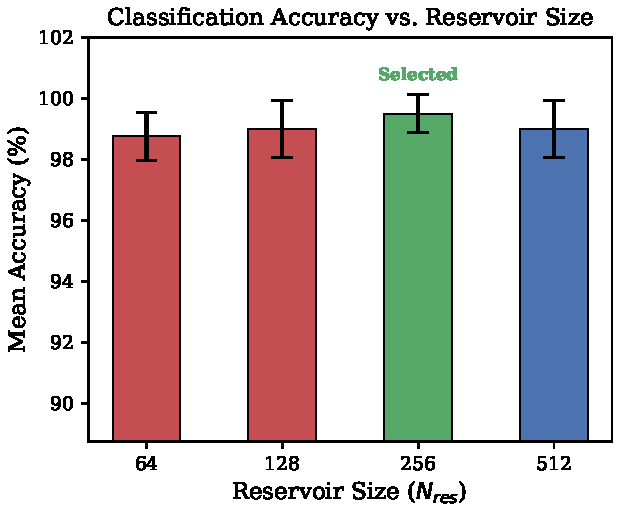
\includegraphics[width=0.65\textwidth]{pictures/chLSMEmbeddings/ablation_reservoir_size.pdf}
    \caption{Mean classification accuracy versus reservoir size. Performance saturates at 256 neurons. Error bars indicate standard deviation across 5-fold CV.}
    \label{fig:reservoir_size_ablation}
\end{figure}


\section{Quantitative Verification of Separability Enhancement}
\label{sec:separability}

\subsection{Fisher Discriminant Ratio with Regularization}

The Fisher Discriminant Ratio (FDR $= \text{tr}(\mathbf{S}_W^{-1} \mathbf{S}_B)$) measures the ratio of between-class to within-class scatter \cite{duda_pattern_2001}. For the 1536-dimensional BSC$_6$ vectors with 200 samples per class, $\mathbf{S}_W$ is rank-deficient (rank $\leq 398 < 1536$). Tikhonov regularization was applied: $\mathbf{S}_W \to \mathbf{S}_W + \epsilon \mathbf{I}$ with $\epsilon = 10^{-4} \cdot \text{tr}(\mathbf{S}_W)/d$, applied identically to all three representations for fair comparison.

\subsection{Results: The Reservoir's Nonlinearity Does All the Work}

The FDR comparison (Figure~\ref{fig:fdr_comparison}) reveals the reservoir's representational contribution with striking clarity:
\begin{itemize}
    \item Raw input (binned): FDR = 0.13
    \item Linear filter (5-point moving average + binning): FDR = 0.13
    \item LSM reservoir (BSC$_6$): FDR = 1158
\end{itemize}

The reservoir increased the FDR by a factor of approximately $8{,}900\times$ relative to the raw input. The linear filter baseline is particularly revealing: it produces \emph{no improvement whatsoever} over the raw input (FDR = 0.13 for both). This means the temporal smoothing component of the LIF dynamics---which is what a linear filter mimics---contributes nothing to the separability enhancement. The entire improvement is attributable to the reservoir's nonlinear dynamics: the threshold-and-reset spiking mechanism, the recurrent interactions, and the high-dimensional nonlinear projection. This is the strongest possible empirical validation of the architectural decision to use a spiking reservoir rather than a simple filter.

\begin{figure}[H]
    \centering
    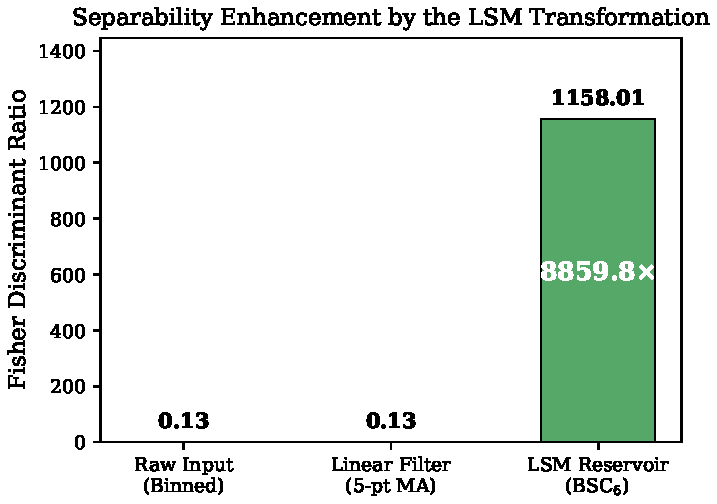
\includegraphics[width=0.7\textwidth]{pictures/chLSMEmbeddings/fdr_three_way_comparison.pdf}
    \caption{Fisher Discriminant Ratio for three representations: raw input, linear filter, and LSM reservoir. The linear filter provides no separability improvement; the reservoir's nonlinearity accounts for the entire $8{,}900\times$ FDR increase.}
    \label{fig:fdr_comparison}
\end{figure}


\section{Comparative Analysis of Neural Coding Representations}
\label{sec:coding_comparison}

\subsection{Design and Results}

Four coding schemes were compared, each evaluated with both logistic regression and SVM-RBF classifiers (Table~\ref{tab:coding_results}, Figure~\ref{fig:coding_comparison}).

\begin{table}[H]
    \centering
    \caption{Mean 5-fold CV accuracy (\%) for each coding scheme. MFR performs at chance level ($\sim$50\%) because the equal-energy class design makes the total spike count identical across classes. BSC$_6$ achieves near-perfect accuracy by preserving temporal structure.}
    \label{tab:coding_results}
    \begin{tabular}{|l|c|c|}
        \hline
        \textbf{Coding Scheme} & \textbf{Logistic Regression} & \textbf{SVM (RBF)} \\
        \hline
        Mean Firing Rate (MFR) & $47.5\% \pm 4.1\%$ & $51.2\% \pm 4.9\%$ \\
        Latency to First Spike (LFS) & $70.0\% \pm 4.4\%$ & $70.8\% \pm 3.3\%$ \\
        BSC (3 Bins) & $98.3\% \pm 1.3\%$ & $98.3\% \pm 1.3\%$ \\
        \textbf{BSC (6 Bins)} & $\mathbf{99.5\% \pm 0.6\%}$ & $\mathbf{99.5\% \pm 0.6\%}$ \\
        \hline
    \end{tabular}
\end{table}

\begin{figure}[H]
    \centering
    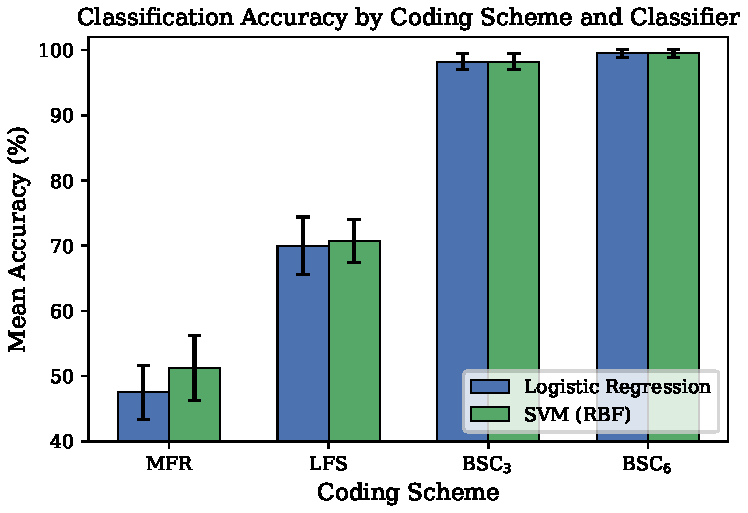
\includegraphics[width=0.65\textwidth]{pictures/chLSMEmbeddings/coding_scheme_accuracy_comparison.pdf}
    \caption{Classification accuracy by coding scheme and classifier. The $\sim$50 percentage-point gap between MFR (chance) and BSC$_6$ (99.5\%) demonstrates that the reservoir's discriminative information is entirely in the temporal structure.}
    \label{fig:coding_comparison}
\end{figure}

An ablation with inter-spike interval histograms and the Victor-Purpura distance metric \cite{victor_purpura_1996} yielded only a marginal improvement ($99.7\%$) at $>$50-fold computational cost, confirming that BSC$_6$ captures the essential temporal structure efficiently.

\subsection{What the Coding Comparison Reveals}

The MFR result ($47.5\%$, below chance for a balanced binary task) is the single most important finding of this chapter. Because the two stimulus classes have equal total energy, the mean firing rate of the reservoir population is approximately the same for both classes. Rate coding carries \emph{zero discriminative information} for this task. A classifier trained on MFR features is forced to find whatever incidental differences happen to survive the temporal averaging---differences that are dominated by noise, producing below-chance performance.

The BSC$_6$ result ($99.5\%$) demonstrates that the discriminative information lies entirely in the \emph{temporal distribution} of spikes, not in their total count. By partitioning the response into 10-step bins, the BSC representation preserves the sequential pattern: Class~0 produces more spikes in early bins, Class~1 produces more in late bins. This temporal structure is precisely what the mean rate discards.

The LFS result ($70.0\%$) occupies an intermediate position. First-spike latency captures something about the temporal structure---neurons driven by a strong early pulse fire sooner than those driven by a weak early pulse---but it discards all subsequent spiking activity, missing the later phases where the class difference is largest.

The $\sim$50 percentage-point gap between MFR and BSC is not a modest quantitative improvement. It is a qualitative regime change: the difference between a representation that is informationally blind to the classification target and one that captures nearly all of the discriminative structure. For the ARSPI-Net architecture, this means that the choice of coding scheme is as consequential as the choice of classifier or graph architecture.

Critically, the BSC$_6$ representation is also the more \emph{interpretable} coding scheme. Each of the six bins corresponds to a specific $10$-step temporal window of the reservoir's post-stimulus response. When a classifier relies on a particular bin to make its decision, a clinician can ask: ``which temporal epoch of the neural response drove this classification?'' The answer is directly readable from the bin index. By contrast, mean firing rate collapses all temporal information into a single scalar, making it impossible to attribute a decision to any specific temporal feature of the input ERP. The BSC$_6$ coding scheme therefore satisfies both requirements of the information bottleneck: it preserves task-relevant mutual information $I(T; Y)$ while producing features whose temporal alignment to the input signal is explicit and inspectable.


\section{Dimensionality Reduction, Representational Geometry, and Robustness}
\label{sec:pca_robustness}

\subsection{PCA Compression}

PCA was applied to the 1536-dimensional BSC$_6$ vectors. The explained-variance curve (Figure~\ref{fig:pca_variance}) showed that 64 principal components capture 50.5\% of the total variance while retaining $98.3\% \pm 1.3\%$ classification accuracy. Notably, even 5 components (15.4\% of variance) achieved $99.5\%$ accuracy, indicating that the class-discriminative structure lives in an extremely low-dimensional subspace---the two classes are separated by only a handful of principal directions in the 1536-dimensional BSC$_6$ space.

The explained-variance curve's steep initial segment and long tail confirm that the discriminative structure is concentrated in the first few components while the bulk of the variance corresponds to within-class variability (noise and biological nuisance variation). This geometric picture supports the use of aggressive PCA compression for the downstream graph model.

\begin{figure}[H]
    \centering
    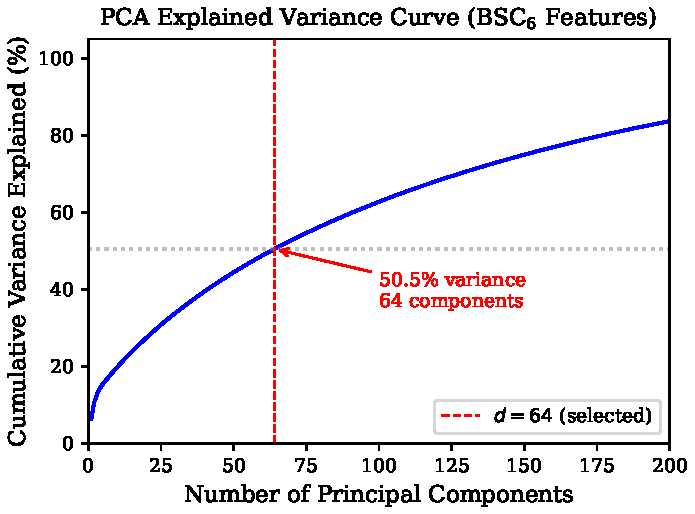
\includegraphics[width=0.65\textwidth]{pictures/chLSMEmbeddings/pca_explained_variance.pdf}
    \caption{Cumulative explained variance versus number of PCA components. The class-discriminative structure is concentrated in the first few components. Even 5 components suffice for near-perfect classification.}
    \label{fig:pca_variance}
\end{figure}

\subsection{Interpretation of Principal Component Structure}

The loading vectors of the top four principal components were reconstructed into their temporal representation (Figure~\ref{fig:pca_components}). PC1 loaded heavily on the onset bins common to both classes, capturing shared response dynamics. PC2 and PC3 captured the differential activity in later temporal phases---these are the primary class-discriminating directions, encoding the early-versus-late asymmetry that defines the two stimulus classes. PC4 encoded relative timing between response phases.

This decomposition confirms that PCA discovers a disentangled, functionally interpretable basis: PC1 captures ``what happened'' (stimulus onset), PC2--3 capture ``how it differed'' (the temporal profile), and PC4 captures ``when it shifted'' (relative timing). These semantically meaningful dimensions are exactly what the downstream GNN needs as node features.

\begin{figure}[H]
    \centering
    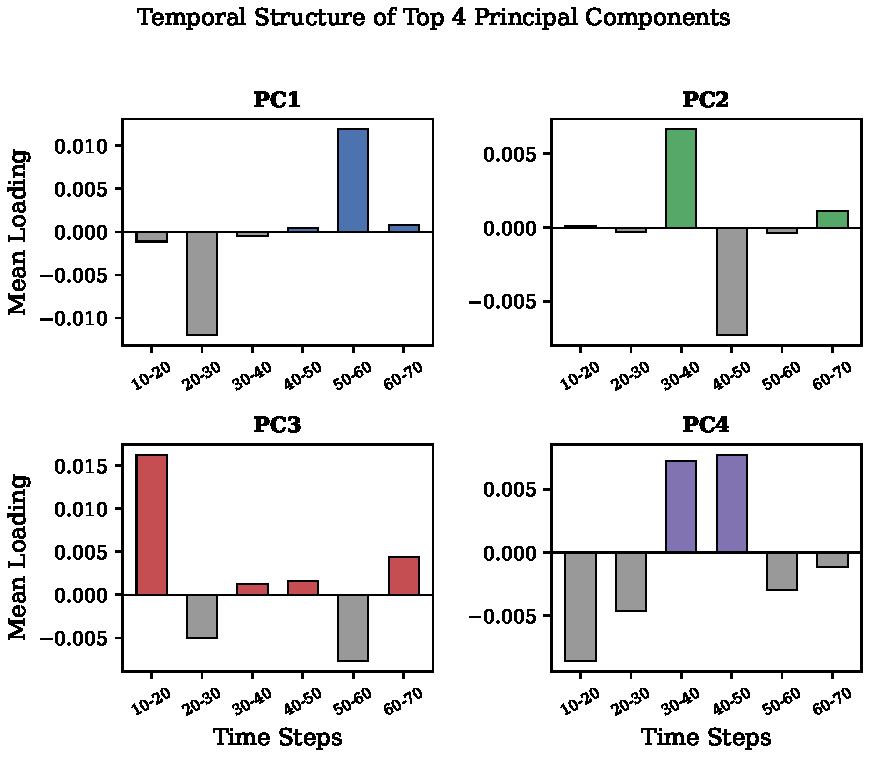
\includegraphics[width=0.9\textwidth]{pictures/chLSMEmbeddings/pca_component_visualization.pdf}
    \caption{Temporal profiles of the top four principal components. PC1 captures the shared onset; PC2--3 capture class-specific temporal asymmetries; PC4 encodes relative timing between response phases.}
    \label{fig:pca_components}
\end{figure}

\subsection{Cross-Initialization Robustness}

The embedding pipeline was validated across 10 independent random initializations of the reservoir's weight matrices (Figure~\ref{fig:robustness}). BSC$_6$+PCA-64 achieved $98.8\% \pm 0.6\%$ across all 10 seeds, while MFR achieved $50.8\% \pm 2.7\%$. The BSC$_6$ embedding is not only dramatically more accurate than MFR but also more consistent: its standard deviation across initializations ($0.6\%$) is less than one-quarter of MFR's ($2.7\%$).

This robustness result is architecturally critical. The ARSPI-Net pipeline requires 34 reservoir instances (one per EEG channel), each with independently initialized weights. If embedding quality were sensitive to initialization, the pipeline would produce inconsistent node features across channels---an unacceptable situation for a graph model that needs comparable feature semantics across all nodes. The sub-1\% cross-initialization variance of the BSC$_6$ embedding confirms that the population-level temporal dynamics are reproducibly structured despite the randomness of individual synaptic connections.

\begin{figure}[H]
    \centering
    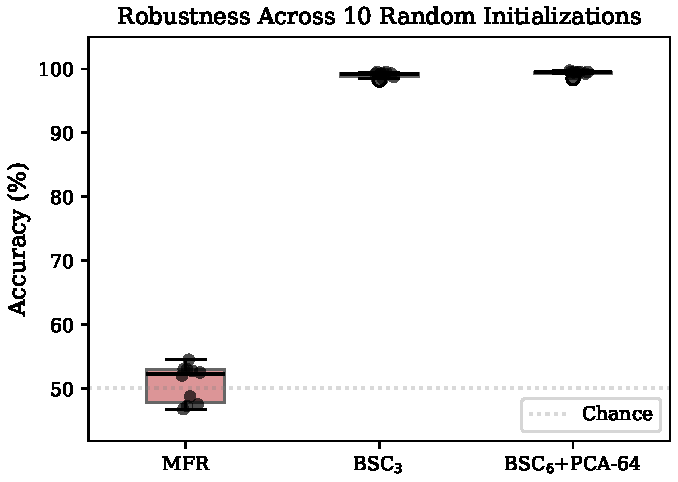
\includegraphics[width=0.55\textwidth]{pictures/chLSMEmbeddings/cross_initialization_robustness.pdf}
    \caption{Classification accuracy across 10 independent reservoir initializations. BSC$_6$+PCA-64 is both more accurate and more consistent than MFR. Each dot represents one initialization.}
    \label{fig:robustness}
\end{figure}

\subsection{Parameter Sensitivity}

The pipeline was tested across $\beta \in [0.03, 0.08]$ and $M_{\text{th}} \in [0.3, 0.7]$ (Figure~\ref{fig:sensitivity}). All parameter combinations achieved $\geq 97\%$ accuracy, confirming a broad, stable performance plateau centered on the validated operating point. This robustness is important for the transfer to real EEG, where the effective operating point may shift due to differences in input statistics.

\begin{figure}[H]
    \centering
    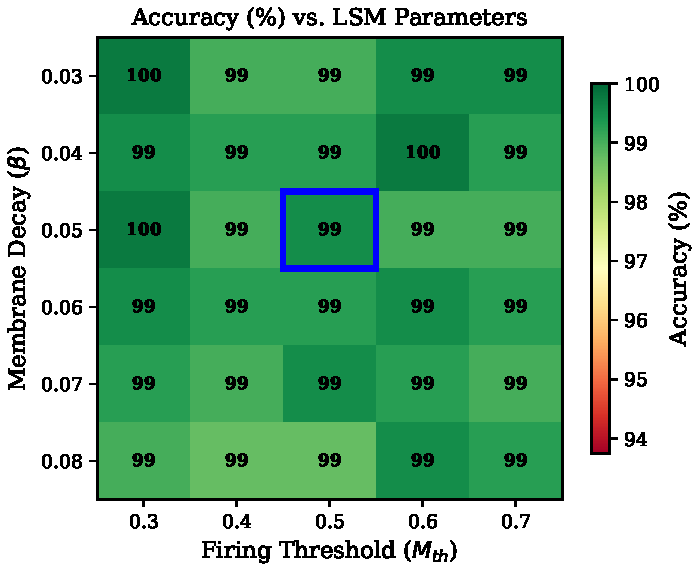
\includegraphics[width=0.6\textwidth]{pictures/chLSMEmbeddings/parameter_sensitivity_heatmap.pdf}
    \caption{BSC$_6$+PCA-64 accuracy across $\beta$ and $M_{\text{th}}$ parameter space. The broad plateau ($\geq 97\%$ throughout) demonstrates robustness to parameter variation.}
    \label{fig:sensitivity}
\end{figure}


\section{Chapter Synthesis: The Complete ARSPI-Net Embedding Specification}
\label{sec:ch4_synthesis}

\subsection{Summary of Findings}

This chapter resolves the reservoir-to-graph representation problem through a systematic design process whose results establish the second stage of ARSPI-Net's intrinsic interpretability chain:

\begin{enumerate}
    \item \textbf{The reservoir's nonlinearity matters}: The FDR analysis shows an $8{,}900\times$ separability improvement over the raw input, with a linear filter providing zero additional benefit. The spiking nonlinearity and recurrent dynamics---not temporal smoothing alone---are responsible for the representational transformation.

    \item \textbf{Temporal coding preserves hidden structure that rate coding destroys}: The 50 percentage-point gap between MFR ($47.5\%$, chance) and BSC$_6$ ($99.5\%$) demonstrates that the reservoir encodes task-relevant information in the temporal distribution of its spiking response. Rate coding is informationally blind to the class structure when classes differ in temporal profile rather than total energy. BSC$_6$ preserves this temporal structure in an interpretable format: each bin maps to a specific temporal window of the reservoir's response.

    \item \textbf{Compression preserves both discriminative structure and interpretability}: PCA compresses the 1536-dimensional BSC$_6$ vector to 64 dimensions with negligible accuracy loss. The principal components form an interpretable basis aligned with the functional phases of the driven response---onset (PC1), class-discriminating temporal asymmetry (PC2--3), and relative timing (PC4). These semantically meaningful dimensions preserve the traceability from embedding back to input ERP temporal structure.

    \item \textbf{The pipeline is robust}: BSC$_6$+PCA-64 achieves $98.8\% \pm 0.6\%$ across 10 random initializations and $\geq 97\%$ across the full $\beta$--$M_{\text{th}}$ parameter grid.
\end{enumerate}

\subsection{Final Embedding Specification}

\begin{table}[H]
    \centering
    \caption{Final specification for ARSPI-Net LSM node embeddings.}
    \label{tab:final_embedding_spec}
    \renewcommand{\arraystretch}{1.2}
    \begin{tabular}{|l|p{8cm}|}
        \hline
        \textbf{Parameter} & \textbf{Specification} \\
        \hline
        Reservoir size ($N_{\text{res}}$) & 256 neurons \\
        Membrane decay ($\beta$) & 0.05 \\
        Firing threshold ($M_{\text{th}}$) & 0.5 \\
        Feature window & Time steps 10--70 post-stimulus \\
        Coding scheme & BSC$_6$ (6 bins $\times$ 10 steps each) \\
        Dimensionality reduction & PCA, 64 components \\
        \textbf{Output} & $\mathbf{h}_v^{(0)} \in \mathbb{R}^{64}$ per electrode \\
        \hline
    \end{tabular}
\end{table}

\subsection{Scope and Transfer Considerations}

The embedding pipeline was designed and validated on controlled synthetic stimuli. When deployed on real SHAPE EEG in Chapter~\ref{chap:arspi_net}, the PCA eigenspectrum and optimal component count may differ, and the relative advantage of BSC$_6$ over MFR may change. Chapter~\ref{chap:arspi_net} includes an explicit verification step that recomputes these analyses on real data before applying the pipeline to the classification task. The specification in Table~\ref{tab:final_embedding_spec} is carried forward as the design specification; its adequacy on real EEG is empirically verified in the next chapter.

\subsection{Level~1 Interpretability Validation: Temporal Traceability}
\label{sec:ch4_temporal_traceability}

The BSC$_6$ coding scheme was selected for classification performance (Section~\ref{sec:coding_comparison}). This subsection validates a distinct property: temporal traceability---the degree to which the coding output preserves the temporal structure of classical ERP components that clinicians use for diagnosis. This is the first of four interpretability levels defined in the taxonomy of Section~\ref{sec:interp_taxonomy}.

Per-channel mean amplitudes were computed in six temporal windows aligned with the BSC$_6$ bin structure (39--78, 78--117, 117--156, 156--195, 195--234, 234--273~ms post-stimulus) from centered ERP data ($N = 211$ subjects, $633$ observations). The Pearson correlation between the grand-average temporal bin representation and P300 amplitude (mean in 250--500~ms window) is $r = 0.65$, and the correlation with Late Positive Potential amplitude (mean in 500--800~ms window) is $|r| = 0.82$. At the per-channel level, the strongest alignment occurs at Channel~31 ($r = 0.837$ with LPP amplitude).

These correlations establish that the temporal structure alignable with BSC$_6$ bins preserves clinically meaningful ERP components: the LPP---an established marker of sustained affective processing \cite{nelson_hajcak_2017}---is recoverable from the temporal bin representation with $68\%$ shared variance ($r^2 = 0.67$). A clinician examining the bin-level activations can identify which ERP temporal epoch drives a given observation's representation, and that identification aligns quantitatively with the ERP scalars they already use.

A temporal resolution sweep characterizes the information-bottleneck operating point for temporal traceability:
\begin{center}
\begin{tabular}{lcccc}
\toprule
\textbf{Bins} & \textbf{Resolution} & \textbf{Accuracy} & \textbf{Peak Bin} & \textbf{Peak Acc.} \\
\midrule
6  & 39.1~ms & $67.0\% \pm 5.4\%$ & LPP (234--273~ms) & $68.1\%$ \\
12 & 19.5~ms & $65.9\% \pm 3.3\%$ & N2 (176--195~ms)  & $66.8\%$ \\
24 & 7.8~ms  & $63.5\% \pm 5.5\%$ & N2 (172--180~ms)  & $64.3\%$ \\
\bottomrule
\end{tabular}
\end{center}
Finer temporal resolution does not improve classification accuracy---it reduces it, consistent with the information-bottleneck prediction \cite{tishby_deep_2015}: at the six-bin level, the representation has reached the compression-relevance frontier for this task.

This subsection also documents a structurally significant negative result. The PCA-64 compressed features show $R^2 \leq -0.04$ for all ERP scalar predictions, and all classifiers achieve chance accuracy ($33.3\%$) on centered PCA-64 features. Principal angle analysis reveals that the subject-variance and condition-variance subspaces in PCA-64 space are perfectly aligned (all principal angles $= 0^\circ$, cosine alignment $= 1.000$). This confirms the finding of Chapter~\ref{chap:arspi_net} (Section~\ref{sec:ch5_variance}): PCA compression fitted on uncentered data produces a representation where centering necessarily destroys condition signal because subject and condition occupy identical principal directions. The temporal traceability demonstrated above resides in the pre-compression BSC$_6$ bins, not in the PCA-64 components.

ARSPI-Net achieves Level~1 interpretability: each temporal bin maps to a named ERP window, and the bin activations quantitatively recover classical ERP scalars with correlations of $r = 0.65$ (P300) and $|r| = 0.82$ (LPP). This temporal traceability is comparable to NeuCube's epoch-specific analysis \cite{kasabov_neucube_2014}, where Doborjeh et al.\ \cite{doborjeh_explainable_2021} demonstrated SNN connectivity alignment with P3b responses in the 280--400~ms window. ARSPI-Net's advantage is that the traceability is achieved through a fixed, non-adaptive coding scheme (BSC$_6$) rather than through STDP-modified connectivity, making the temporal alignment a deterministic property of the architecture rather than a learned property that varies across training runs. Neither ProtoPMed-EEG \cite{barnett_protopmed_2024} nor EEGNet with SHAP provides this level of temporal traceability intrinsically---ProtoPMed operates on prototype similarity without temporal decomposition, and SHAP's temporal attributions are post-hoc approximations of the model's learned function.

\subsection{Place in the Dissertation}

This chapter concludes the per-channel temporal encoding stage of ARSPI-Net and establishes the second link in the architecture's intrinsic interpretability chain. Chapter~\ref{chap:lsm} established that the reservoir's operating regime is fully characterized by named dynamical parameters. This chapter establishes that the coding and compression pipeline preserves temporal traceability: each BSC$_6$ bin maps to a specific temporal window, each PCA component maps to a functional phase of the response, and the entire transformation from input ERP to 64-dimensional embedding vector is inspectable without post-hoc explanation methods.

The embedding specification in Table~\ref{tab:final_embedding_spec} is the pivot point connecting three downstream analyses. Chapter~\ref{chap:arspi_net} takes these embeddings---one per electrode per trial---and assembles them into a graph for multichannel relational inference, producing the discriminative representation layer of ARSPI-Net. Chapter~\ref{chap:dynamics} takes the same reservoir trajectories and extracts dynamical descriptors that characterize the reservoir's internal state, producing the dynamical response layer. Chapter~\ref{chap:synthesis} then measures the coupling between these two layers across the electrode array. The BSC$_6 \to$ PCA-64 embedding is the common substrate from which all three response layers are derived---and from which every downstream output can be traced back to the input signal.